% !TeX spellcheck = pl_PL

\newpage
\part{Zadania}
% ==================================================
% --- TOPOLOGIA SIECI
% ==================================================
\section{Topologia sieci}
	% ================= ZADANIE 1 ==================
	\subsection{Zadanie}
		\subsubsection{Treść}
			\begin{wrapfigure}{l}{6.0cm}
				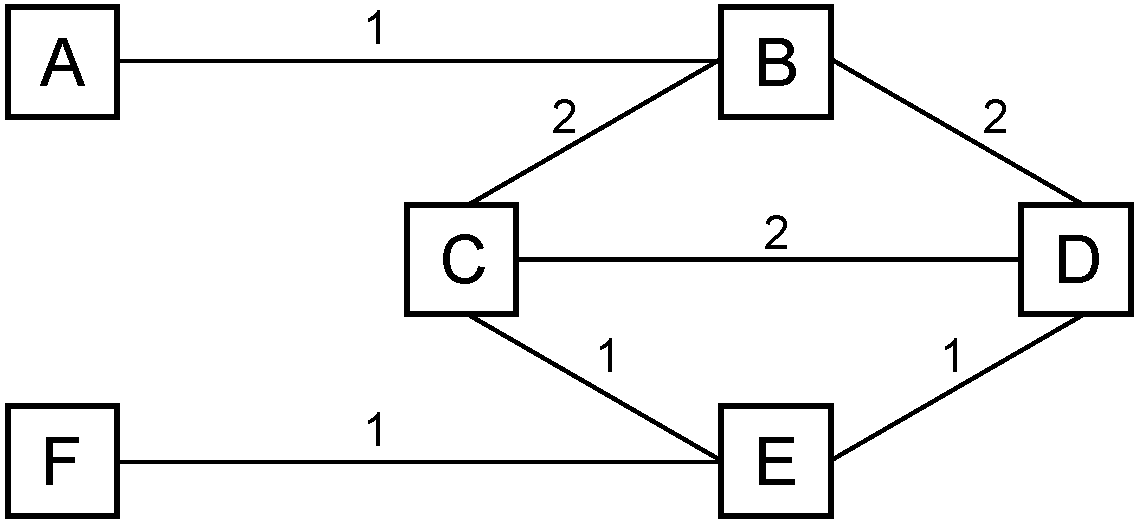
\includegraphics[width=5.5cm]{./images/zadanie02.pdf}
			\end{wrapfigure} 
			W sieci z metryką jak na rysunku routery wymieniają się informacjami co 40 sekund, stosowany jest protokół typu Distance Vector. W chwili $ t_0 $ router F ulega awarii. Określ, po jakim czasie informacja o niedostępności routera F dotrze do węzła A.\\\\\\\\
		\subsubsection{Odpowiedź}
			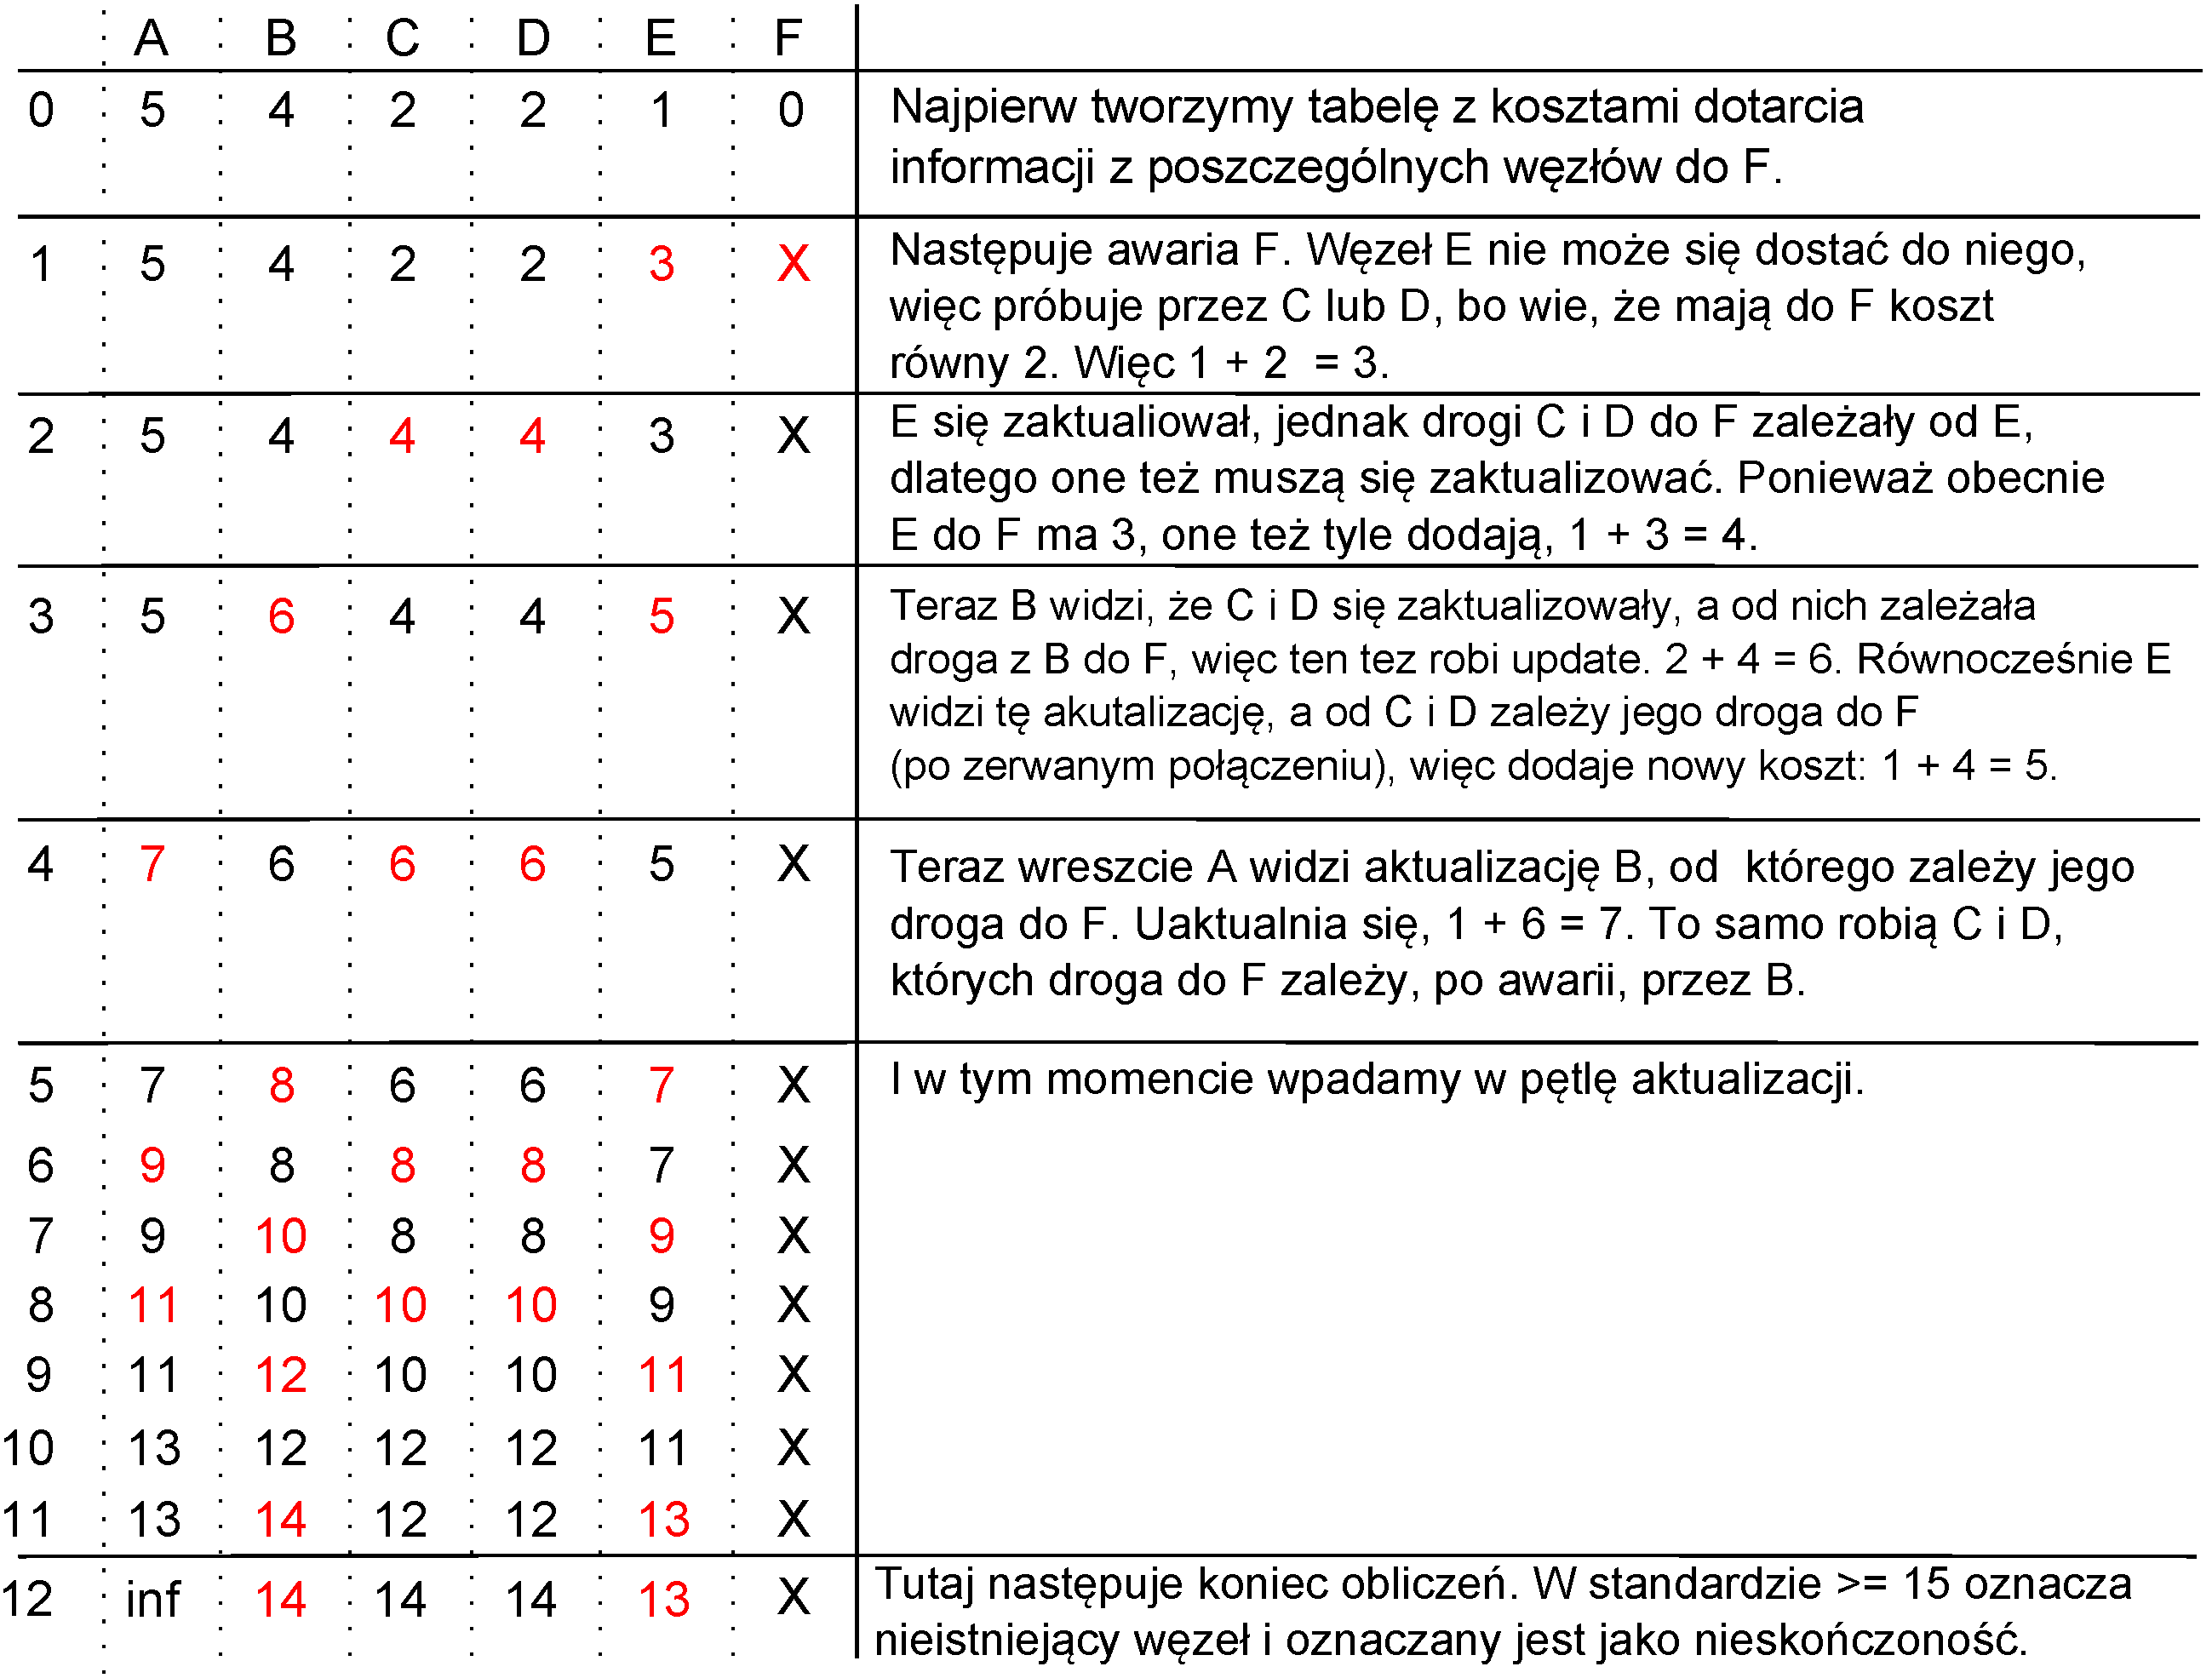
\includegraphics[width=11.0cm]{./images/zadanie03.pdf}\\
			A więc stacja A dowie się o niedostępności stacji F po $ 12\cdot 40\;s=480\;s $.
	% ================= ZADANIE 2 ==================
	\subsection{Zadanie}
		\subsubsection{Treść}
			Dana jest następująca topologia sieci:
			\begin{itemize}
				\item Węzeł B ma jako sąsiadów węzły A, C i D
				\item Węzeł C ma jako sąsiadów węzły A, B, D i E
				\item Węzeł D ma jako sąsiadów węzły A, B, C i E
				\item Węzeł E ma jako sąsiadów węzły C i D
			\end{itemize}
			W chwili $ t_0 $ węzeł B ulega awarii. Przedstaw sposób rozchodzenia się tej informacji między węzłami, po jakim czasie informacja o tym dotrze do węzła E, jeśli w sieci stosowany jest protokół RIP typu Distance Vector i cykl wymiany wektorów wynosi 30 s. Przyjmij metrykę jednostkową łączy.
		\subsubsection{Odpowiedź}
			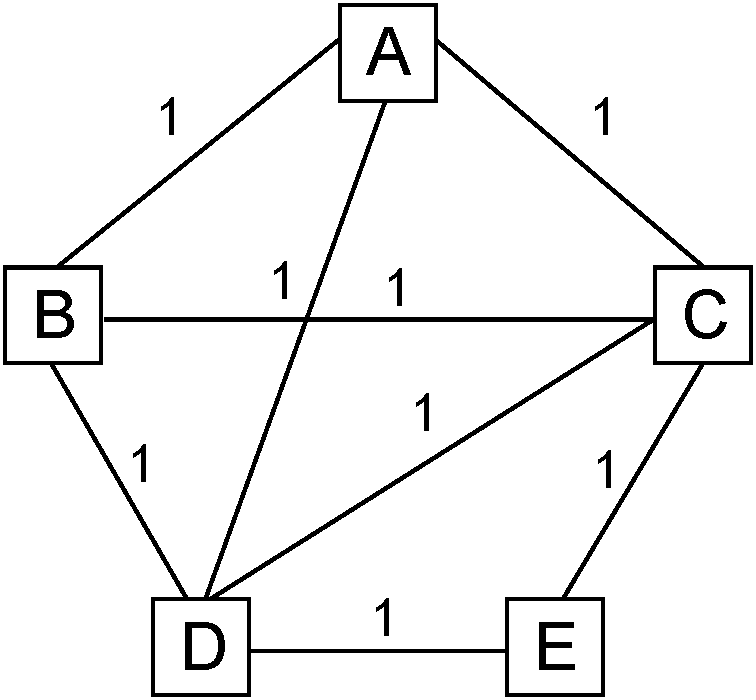
\includegraphics[width=5.0cm]{./images/zadanie04.pdf}\\\\
			\begin{tabular}{|c|c|c|c|c|c|p{7cm}|}
				\hline \textbf{Zmiana} & \textbf{A} & \textbf{B} & \textbf{C} & \textbf{D} & \textbf{E} & \textbf{Komentarz} \\ 
				\hline \textbf{-} & 1 & 0 & 1 & 1 & 2 & Działa \\ 
				\hline \textbf{0} & \color{red}{inf} & \color{red}{X} & \color{red}{inf} & \color{red}{inf} & 2 & B ulega awarii. Sąsiedzi, czyli A, C i D nie mogą się połączyć z nim. \\ 
				\hline \textbf{1} & \color{red}{4} & X & \color{red}{3} & \color{red}{3} & 2 & Węzły A, B i C próbują się połączyć z B przez E, który nie wie o awarii. \\ 
				\hline \textbf{2} & 4 & X & 3 & 3 & \color{red}{4} & Ponieważ droga z węzła E do B pierwotnie wiodła przez węzły D i C, po ich zmianie ich tablic, E również musi je aktualizować, nawet pomimo tego, że obecna droga C i D wiedzie przez niego (nie wie o tym). \\
				\hline \textbf{3} & \color{red}{6} & X & \color{red}{5} & \color{red}{5} & 4 & I zaczyna się pętla. \\ 
				\hline \textbf{4} & 6 & X & 5 & 5 & \color{red}{6} &  \\ 
				\hline \textbf{5} & \color{red}{8} & X & \color{red}{7} & \color{red}{7} & 6 &  \\ 
				\hline \textbf{6} & 8 & X & 7 & 7 & \color{red}{8} &  \\ 
				\hline \textbf{7} & \color{red}{10} & X & \color{red}{9} & \color{red}{9} & 8 &  \\ 
				\hline \textbf{8} & 10 & X & 9 & 9 & \color{red}{10} &  \\ 
				\hline \textbf{9} & \color{red}{12} & X & \color{red}{11} & \color{red}{11} & 10 &  \\ 
				\hline \textbf{10} & 12 & X & 11 & 11 & \color{red}{12} &  \\ 
				\hline \textbf{11} & \color{red}{14} & X & \color{red}{13} & \color{red}{13} & 12 &  \\ 
				\hline \textbf{12} & 14 & X & 13 & 13 & \color{red}{14} &  \\ 
				\hline \textbf{13} & \color{red}{16} & X & \color{red}{15} & \color{red}{15} & 14 &  \\ 
				\hline \textbf{14} &  &  &  &  & \color{red}{16} & Koniec \\ 
				\hline 
			\end{tabular}\\\\
			Obliczenia kończą się, gdy koszt trasy z węzła E do B przekroczy 15. Wówczas widzimy, że dokonanych zmian było 14, a więc czas wynosi: $ 14\cdot 30\;s=420\;s=7$ minut.

% ==================================================
% --- ETHERNET
% ==================================================
\section{Ethernet}
	% ================= ZADANIE 1 ==================
	\subsection{Zadanie}
		\subsubsection{Treść}
			Kontroler karty sterownika sieci Ethernet odebrał następujące ramki:
			\begin{enumerate}
				\item Długość 51 bajtów, poprawne CRC
				\item Długość 39 bajtów, błędne CRC
				\item Długość 66 bajtów, poprawne CRC
				\item Długość 1510 bajtów, poprawne CRC
				\item Długość 1525 bajtów, poprawne CRC
				\item Długość 1540 bajtów, błędne CRC
			\end{enumerate}
			Jak zaklasyfikować powyższe ramki? (błąd protokołu, błąd transmisji, kolizja, poprawna ramka)
		\subsubsection{Odpowiedź}
			\begin{itemize}
				\item Jeśli ramka ma mniej niż 64 bajty i błędne CRC to jest to kolizja
				\item Jeśli ramka ma mniej niż 64 bajty i poprawne CRC to jest to błąd protokołu
				\item Jeśli ramka ma więcej niż 1518 bajtów, to zawsze jest to błąd protokołu, niezależnie od poprawności CRC
				\item Jeśli ramka ma niemniej 64 bajty i nie więcej niż 1518 bajtów oraz niepoprawne CRC to jest to błąd transmisji
				\item Poprawna ramka powinien mieć 64 - 1518 bajtów i poprawne CRC
			\end{itemize}
			\begin{enumerate}
				\item Błąd protokołu
				\item Kolizja
				\item Poprawna
				\item Poprawna
				\item Błąd protokołu
				\item Błąd protokołu
			\end{enumerate}
	% ================= ZADANIE 2 ==================
	\subsection{Zadanie}
		\subsubsection{Treść}
			W przypadku wystąpienia kolizji w segmencie sieci Ethernet czas oczekiwania na retransmisję $ T_R $ generowany jest jako liczba losowa z przedziału:
			\begin{enumerate}
				\item O stałej wielkości ustalanej przy konfiguracji sieci (jakiej?)
				\item O wielkości rosnącej liniowo z numerem kolizji
				\item O wielkości rosnącej z kwadratem numeru kolizji
				\item O wielkości rosnącej z kwadratem do pewnego numeru kolizji
			\end{enumerate}
			Jak obliczany jest czas $ T_R $?
		\subsubsection{Odpowiedź}
			Chodzi tutaj o algorytm CSMA, wykorzystywany do rozwiązywania kolizji na łączu kablowym. Wzór, o który prosi pytanie, zawarty jest w algorytmie dostępu w transmisji częściowo kontrolowanej. W pełni kontrolowanym dostępie występuje Token oraz rywalizacja stacji o dostęp (chyba o to chodzi).
			$$ T_{R} = r(x)\times (2^{k}-1)\times T_{ob}$$Gdzie:
			\begin{itemize}
				\item $ r(x) $ - liczba losowa z zakresu 0...1
				\item $ T_{ob} $ - czas obiegu łącza, w najgorszym wypadku podwojony czas propagacji
				\item $ k $ - liczba kolizji, czyli który raz się te ramki już zderzyły.
				\item Wraz ze zwiększaniem się liczby kolizji, możliwy zakres rośnie ekspotencjalnie. Jednak maksymalna wielkość $ k $ jest równa \textbf{10}. Dla $ k > 10 $ przyjmuje się $ k=10 $.
				\item Próbujemy szczęścia aż $ k < 15 $, potem próby są przerywane.
			\end{itemize}
			Dlatego poprawna odpowiedź to: \textit{Czas oczekiwania na retransmisję $ T_R $ generowany jest jako liczba losowa z przedziału \textbf{o wielkości rosnącej z kwadratem do pewnego numeru kolizji, \underline{a tym numerem jest 10}}}\\
			{\small \emph{Forczu: jeszcze to sprawdzę}}.
			
% ==================================================
% --- TCP / IP
% ==================================================
\section{TCP / IP}
% ================= ZADANIE 1 ==================
\subsection{Zadanie}
	\subsubsection{Treść}
		Przedstaw i porównaj dostępne mechanizmy działania protokołu sterowania przypływem w połączeniach warstwy transportowej i w połączeniach warstwy liniowej (np. SDLC, TCP). W jaki sposób odbierająca stacja transportowa może uzyskać czasowe powstrzymanie transmisji przez nadawcę?
	\subsubsection{Odpowiedź}
		\begin{itemize}
			\item \textbf{TCP} - kontrolowanie poprzez zmianę rozmiaru okna odbiorcy.
			\item \textbf{SDLC / HDLC} - kontrolowanie przez sygnały typu WACK / ACK w protokole znakowym BSC (RR, RNR).
		\end{itemize}
	
% ==================================================
% --- ROUTING
% ==================================================
\section{Routing}
	% ================= ZADANIE 1 ==================
	\subsection{Zadanie}
		\subsubsection{Treść}
			\begin{wraptable}{r}{5.5cm}
				\begin{tabular}{|c|c|}
					\hline \multicolumn{2}{|c|}{Q}  \\ 
					\hline \multicolumn{2}{|c|}{1}  \\ 
					\hline \multicolumn{2}{|c|}{300}  \\ 
					\hline T & 2 \\ 
					\hline U & 1 \\ 
					\hline Z & 3 \\ 
					\hline 
				\end{tabular}
			\end{wraptable}
			Węzeł Q generuje co 60 sekund pakiety Link State, w chwili $ t_0 $ rozesłał pakiet
			$$ (Q\;|\;seq=23321\;|\;age=300\;|\;(U|3)\;|\;(V|2)\;|\;(Z|5)\;) $$
			Po restarcie w chwili $ t_0+25\;s $ wysłał pakiet
			$$ (Q\;|\;seq=1\;|\;age=300\;|\;(T|2)\;|\;(U|1)\;|\;(Z|3)\;) $$
			a potem kolejne. Przedstaw przebieg dystrybucji tej informacji w sieci. Kiedy te zmiany w topologii zostaną uwzględnione w wyznaczaniu tablicy routingu?
		\subsubsection{Odpowiedź}
			Działanie Link State:
			\begin{itemize}
				\item "Powiedz wszystkim o swoich sąsiadach" - przekazuje pakiety otrzymane od sąsiednich węzłów do sąsiednich węzłów.
				\item Nr sekwencyjny - jeśli ktoś dostanie pakiet o większym numerze, to go przetwarza (i przesyła dalej), a jeśli nie jest większy, to nie.
				\item Wiek - czas życia pakietu (w cyklu). Jeśli czas życia upływa to jest usuwany z tablicy routingu. Liczony w sekundach.
			\end{itemize}
			\textbf{Odpowiedzi}:
			\begin{enumerate}
				\item Węzły odrzucają pakiet z niższym numerem sekwencyjnym, więc nowy pakiet będzie uwzględniony po wygaśnięciu wa(żności?) pierwszego, czyli za $ 275\;s $.\\
				\small{ \emph{Ocenione na 0.9 / 1.0}}
				\item \small{ \emph{Forczu:}} dlaczego ujebano ten 0.1? Wg mnie dlatego, że kruczek tkwi w słowie "reset". Pakiety są wysyłane co 60 sekund, ale od momentu resetu ($ t_0+25\;s $) zaczynamy liczyć od nowa, czyli nowe pakiety są wysyłane w momentach $ 85\;s, 145\;s, 205\;s $ itd.\\
				Dlatego prawidłową odpowiedzią imo jest $ t_0+25+\textbf{6}\cdot{60}=325\;s $, czyli dopiero 6ty pakiet zostanie uwzględniony przez tablicę routingu.
				\item \small{ \emph{Inna odpowiedź, ocena nienzna:}}\\
				W momencie restartu, po 25 sekundach, oba pakiety żyją i ważniejszy jest Pierwszy z nich, o numerze sekwencyjnym $ seq=23321 $. Dlatego pakiet o $ seq=1 $ zostanie uwzględniony po przedawnieniu $ seq=23321 $, czyli po:
				$$ 300 - 25 - t_0\;[s]= 275\;[s] $$
				a najpierw zostanie wykorzystany pakiet o $ seq=23321 $.
				\item \emph{by Forczu}: tablica po uwzględnieniu pakiet o $ seq=23321 $ \\
					\begin{tabular}{|c|c|}
						\hline \multicolumn{2}{|c|}{Q}  \\ 
						\hline \multicolumn{2}{|c|}{1}  \\ 
						\hline \multicolumn{2}{|c|}{300}  \\ 
						\hline T & 2 \\ 
						\hline U & 1 \\
						\hline V & 2 \\
						\hline Z & 3 \\ 
						\hline 
					\end{tabular}\\\\
				Nowe $ U=3 $, czyli koszt jest wyższy od obecnego, więc nie jest uwzględnione.\\
				Nowe $ Z=5 $, czyli to samo co wyżej.\\
				Nowe $ V=5 $, tego nie ma w obecnej tablicy, więc po prostu jest dodane.
		\end{enumerate}
	% ================= ZADANIE 2 ==================
	\subsection{Zadanie}
		\subsubsection{Treść}
			Węzeł D odebrał / wysłał do chwili $ T_0 $ następujące pakiety.\\
			\begin{tabular}{|c|c|c|c|c|c|c|c|c|c|c|c|c|c|c|c|c|c|c|c|c|c|c|c|c|c|c|c|c|}
				\cline{1-2} \cline{4-5} \cline{7-8} \cline{10-11} \cline{13-14} \cline{16-17} \cline{19-20} \cline{22-23} \cline{25-26} \cline{28-29}
				\multicolumn{2}{|c|}{G} &  & \multicolumn{2}{c|}{B}  &  & \multicolumn{2}{c|}{C} &  & \multicolumn{2}{c|}{E}  &  & \multicolumn{2}{c|}{D}  &  & \multicolumn{2}{c|}{F}  &  & \multicolumn{2}{c|}{A}  &  & \multicolumn{2}{c|}{H}  &  & \multicolumn{2}{c|}{C}  &  & \multicolumn{2}{c|}{B} \\ \cline{1-2} \cline{4-5} \cline{7-8} \cline{10-11} \cline{13-14} \cline{16-17} \cline{19-20} \cline{22-23} \cline{25-26} \cline{28-29} 
				\multicolumn{2}{|c|}{9} &  & \multicolumn{2}{c|}{8}  &  & \multicolumn{2}{c|}{9} &  & \multicolumn{2}{c|}{8}  &  & \multicolumn{2}{c|}{9}  &  & \multicolumn{2}{c|}{14} &  & \multicolumn{2}{c|}{10} &  & \multicolumn{2}{c|}{9}  &  & \multicolumn{2}{c|}{10} &  & \multicolumn{2}{c|}{7} \\ \cline{1-2} \cline{4-5} \cline{7-8} \cline{10-11} \cline{13-14} \cline{16-17} \cline{19-20} \cline{22-23} \cline{25-26} \cline{28-29} 
				\multicolumn{2}{|c|}{3} &  & \multicolumn{2}{c|}{25} &  & \multicolumn{2}{c|}{7} &  & \multicolumn{2}{c|}{28} &  & \multicolumn{2}{c|}{29} &  & \multicolumn{2}{c|}{21} &  & \multicolumn{2}{c|}{23} &  & \multicolumn{2}{c|}{24} &  & \multicolumn{2}{c|}{23} &  & \multicolumn{2}{c|}{6} \\ \cline{1-2} \cline{4-5} \cline{7-8} \cline{10-11} \cline{13-14} \cline{16-17} \cline{19-20} \cline{22-23} \cline{25-26} \cline{28-29} 
				F          & 1          &  & A           & 3         &  & B          & 1         &  & A           & 1         &  & C           & 2         &  & A           & 1         &  & E           & 1         &  & B           & 1         &  & B           & 3         &  & A          & 1         \\ \cline{1-2} \cline{4-5} \cline{7-8} \cline{10-11} \cline{13-14} \cline{16-17} \cline{19-20} \cline{22-23} \cline{25-26} \cline{28-29} 
				H          & 1          &  & H           & 2         &  & E          & 2         &  & C           & 2         &  & H           & 1         &  & E           & 1         &  & B           & 2         &  & G           & 2         &  & E           & 1         &  & H          & 1         \\ \cline{1-2} \cline{4-5} \cline{7-8} \cline{10-11} \cline{13-14} \cline{16-17} \cline{19-20} \cline{22-23} \cline{25-26} \cline{28-29} 
				D          & 1          &  & C           & 2         &  & D          & 2         &  & F           & 1         &  & G           & 1         &  & G           & 1         &  & F           & 2         &  & D           & 2         &  & D           & 1         &  & C          & 2         \\ \cline{1-2} \cline{4-5} \cline{7-8} \cline{10-11} \cline{13-14} \cline{16-17} \cline{19-20} \cline{22-23} \cline{25-26} \cline{28-29}
				\multicolumn{2}{c}{1} &  & \multicolumn{2}{c}{2} &  & \multicolumn{2}{c}{3} &  & \multicolumn{2}{c}{4} &  & \multicolumn{2}{c}{5} &  & \multicolumn{2}{c}{6} &  & \multicolumn{2}{c}{7} &  & \multicolumn{2}{c}{8} &  & \multicolumn{2}{c}{9} &  & \multicolumn{2}{c}{10} \\ 
			\end{tabular}\\
			W czasie $ T_0+5 $ węzeł D rozpoczął wyznaczanie nowej tablicy routingu. Przedstawić nową tablicę routingu dla węzła D.
		\subsubsection{Odpowiedź}
			Format pakiety wyraźnie wskazuje, że mamy do czynienia z algorytmem Link State.
			\begin{itemize}
				\item Pierwsza wartość oznacza nadawcę.
				\item Druga wartość to numer sekwencyjny - im większy tym pakiet jest ważniejszy.
				\item Trzecia wartość to wiek - po tego upływie czasu od momentu odebrania pakiet jest usuwany.
			\end{itemize}
			Tak więc na samym początku \textbf{odrzucamy} pakiety nr 1 o czasie życia 3 - w momencie wyznaczania nowej tablicy, w momencie $ T_0+5 $ już nie istniał.\\
			Następnie patrzymy na numery sekwencyjne - jeżeli odebraliśmy 2+ pakietów od tego samego węzła, to interesuje nas tylko ten o najwyższym numerze sekwencyjnym.
			\begin{itemize}
				\item Są dwa pakiety od węzła B, nr 2 i 10. Odrzucamy nr 10 o niższym \textit{seq} ($ 8 > 7 $).
				\item Są dwa pakiety od węzła C, nr 3 i 9. Odrzucamy nr 3 o niższym \textit{seq} ($ 9 < 10 $).
			\end{itemize}
			Do obliczeń przystępujemy z 7 pakietami. Wszystko sobie rozrysowujemy:\\
			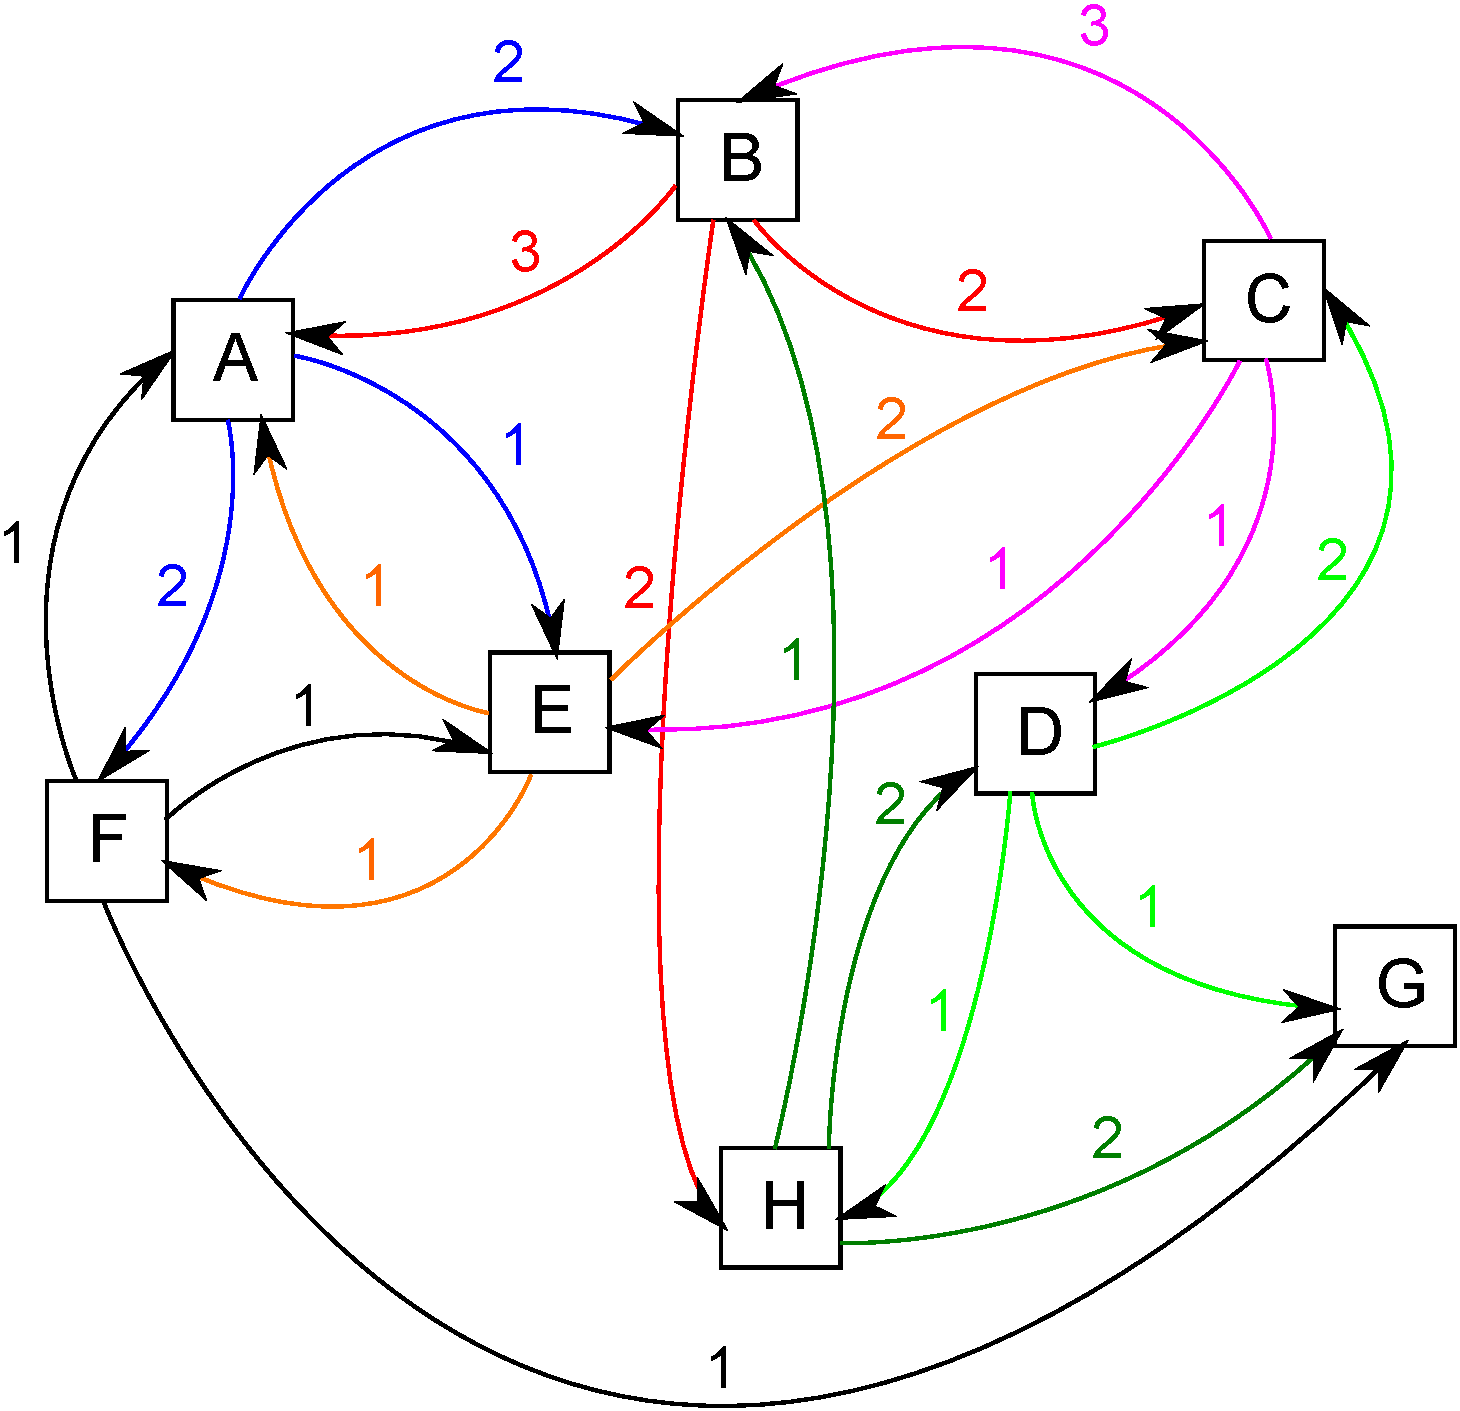
\includegraphics[width=7.0cm]{./images/zadanie05.pdf}\\
			Jeśli węzły da się połączyć na dwa różne sposoby, tworzymy średnią arytmetyczną. Wybieramy najkrótsze możliwe połączenie do każdego węzła, \textbf{pomijamy G}, i rysujemy tabelkę.\\\\
			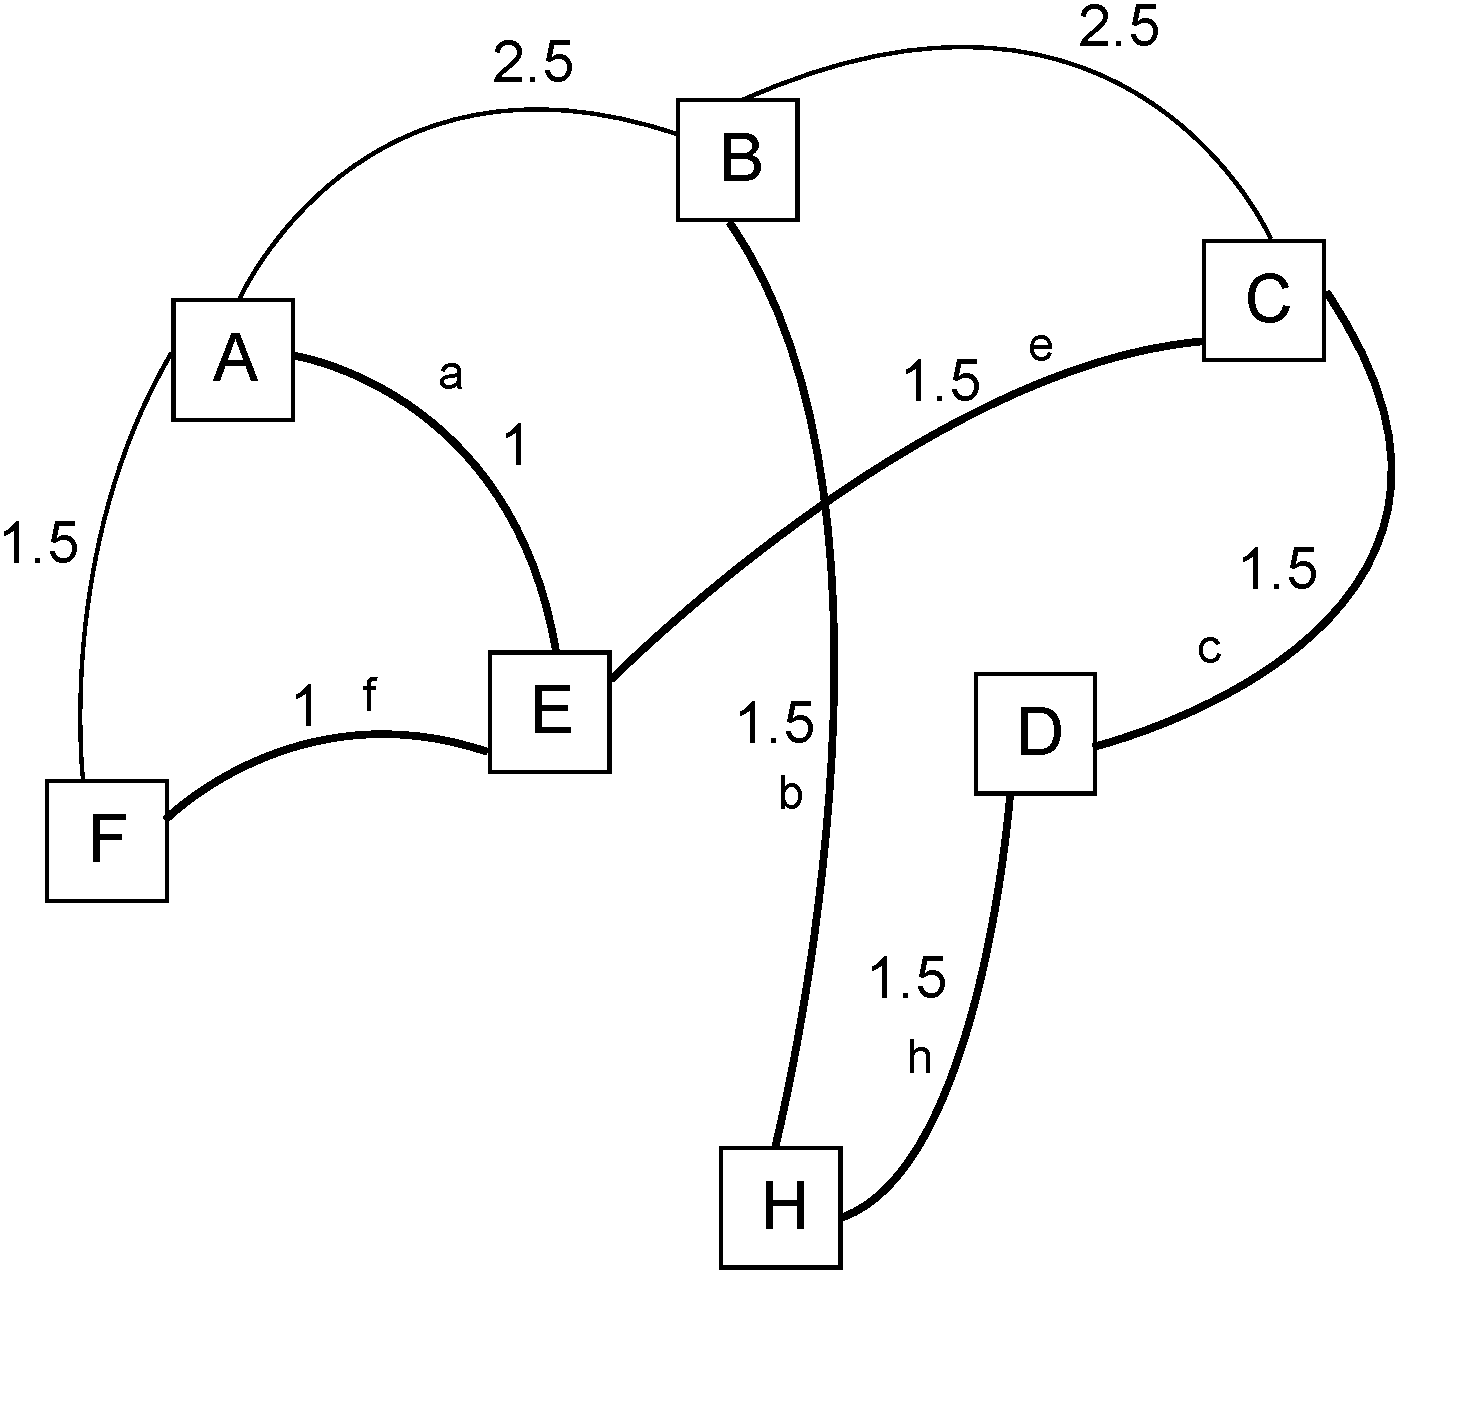
\includegraphics[width=7.0cm]{./images/zadanie06.pdf}     
			\begin{tabular}{c|c|c}
				Cel & Koszt & Przez \\ \hline
				A   & 4     & E     \\
				B   & 3     & H     \\
				C   & 1.5   & D     \\
				D   & 0     &       \\
				E   & 3     & C     \\
				F   & 4     & E     \\
				G   & -     &       \\
				H   & 1.5   & D     
			\end{tabular}\\
			\small{ \emph{Forczu: ocenione na 1.0 / 1.0}}.
	% ================= ZADANIE 2 ==================
	\subsection{Zadanie}
		\subsubsection{Treść}
			Węzeł K po restarcie wysłał do sąsiadów L, I, F swoją początkową tablicę routingu i otrzymał od nich ich tablice routingu. Wyznacz nową tablicę routingu węzła K.\\\\
			\begin{tabular}{cc m{1cm}|c|c|c|c|c|ccc}
				\cline{1-2} \cline{4-5} \cline{7-8} \cline{10-11}
				\multicolumn{2}{|c|}{\textbf{K}}                 &  & \multicolumn{2}{c|}{\textbf{L}} &  & \multicolumn{2}{c|}{\textbf{F}} & \multicolumn{1}{c|}{} & \multicolumn{2}{c|}{\textbf{I}}                 \\ \cline{1-2} \cline{4-5} \cline{7-8} \cline{10-11} 
				\multicolumn{1}{|c|}{I} & \multicolumn{1}{c|}{1} &  & D              & 3              &  & A              & 3              & \multicolumn{1}{c|}{} & \multicolumn{1}{c|}{J} & \multicolumn{1}{c|}{2} \\ \cline{1-2} \cline{4-5} \cline{7-8} \cline{10-11} 
				\multicolumn{1}{|c|}{F} & \multicolumn{1}{c|}{2} &  & C              & 4              &  & B              & 2              & \multicolumn{1}{c|}{} & \multicolumn{1}{c|}{H} & \multicolumn{1}{c|}{3} \\ \cline{1-2} \cline{4-5} \cline{7-8} \cline{10-11} 
				\multicolumn{1}{|c|}{L} & \multicolumn{1}{c|}{1} &  & G              & 2              &  & C              & 1              & \multicolumn{1}{c|}{} & \multicolumn{1}{c|}{N} & \multicolumn{1}{c|}{3} \\ \cline{1-2} \cline{4-5} \cline{7-8} \cline{10-11} 
				&                        &  & H              & 1              &  & E              & 2              & \multicolumn{1}{c|}{} & \multicolumn{1}{c|}{M} & \multicolumn{1}{c|}{4} \\ \cline{4-5} \cline{7-8} \cline{10-11} 
				&                        &  & N              & 2              &  & G              & 1              & \multicolumn{1}{c|}{} & \multicolumn{1}{c|}{E} & \multicolumn{1}{c|}{3} \\ \cline{4-5} \cline{7-8} \cline{10-11} 
				&                        &  & M              & 5              &  & J              & 2              &                       &                        &                        \\ \cline{4-5} \cline{7-8}
			\end{tabular}
		\subsubsection{Odpowiedź}
		\begin{wraptable}{l}{5.5cm}
			\begin{tabular}{c|c|c}
				Do & Przez & Koszt \\ \hline
				A  & F     & 5     \\
				B  & F     & 4     \\
				C  & F     & 3     \\
				D  & L     & 4     \\
				E  & F     & 4     \\
				F  & -     & 2     \\
				G  & L     & 3     \\
				H  & L     & 2     \\
				I  & -     & 1     \\
				J  & I     & 3     \\
				K  & -     & -     \\
				L  & -     & 1     \\
				M  & I     & 5     \\
				N  & L     & 3    
			\end{tabular}
		\end{wraptable}
		W tym wszystkim interesują nas tylko drogi lokalnie najbliższe - te z punktu widzenia węzła K i "ofert" dróg sąsiadów. Jeśli dwie drogi mają ten sam koszt to wybór powinien być obojętny. Sąsiedzi (L, I, D) mają się w końcowej tabeli również znajdować.\\
		\small{ \emph{Forczu: ocenione na 1.0 / 1.0}}.\\\\\\\\\\\\\\\\\\\\\\\\
\section{Transmisja danych}
% ================= ZADANIE 1 ==================
	\subsection{Zadanie}
		\subsubsection{Treść}
			Stacja robocza połączona jest z serwerem łączem szeregowym o przepustowości 8 MBit/s, z bitową stopą błędów $ BER=2\cdot 10^{-5} $. Określić z jaką średnią szybkością transmisji danych protokołem TCP w wersji standardowej (\emph{plain vanilla}) można uzyskać jeśli uzgodniona maksymalna wielkość segmentu wynosi 768 B (ramki w łączu 832 B), wielkość danych odbiorcy wynosi 27 kB, czas $ RTT=40\;ms $.
		\subsubsection{Odpowiedź}
			$ BER=2\cdot 10^{-5} \rightarrow 50000 $ - oznacza to, że 1 na 50k bitów jest przekłamany, czyli co 6250 bajt jest przekłamany.\\\\
			$ V=8 Mb/s $\\\\
			$ \cfrac{6250\;[B]}{832\;[B]}=7.51 \rightarrow$ co 7.51 ramka jest przekłamana.\\
			Teraz stosujemy metodę słupków do wyznaczenia właściwego stosunku liczby ramek, jakie można wysłać. Rysujemy kolejne transmitowane ramki w postaci słupków złożonych z $ 2^n $ ramek: 1, 2, 4, 8 itd. Gdy napotykamy przekłamaną ramkę zaczynamy naliczać od nowa. Kończymy naliczanie gdy przekłamana ramka znajdzie się na szczycie jednego ze słupków.Oznacza ona bowiem zakończenie cyklu, "deja vu" - kolejne kolumny, wraz z przekłamaniami, będą się powtarzać.\\\\
			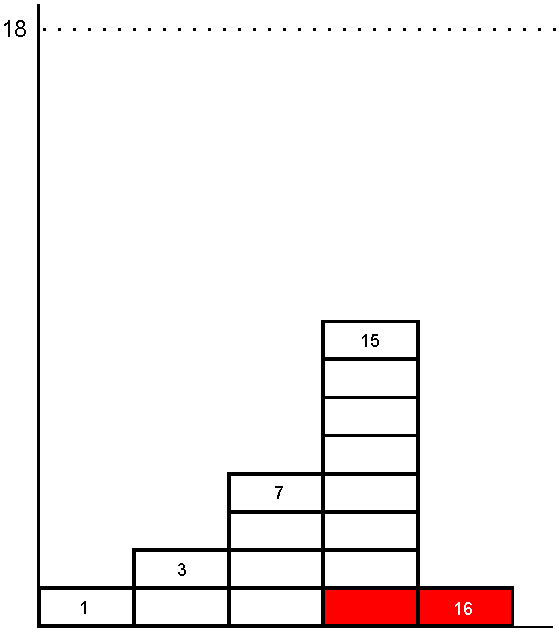
\includegraphics[width=5.0cm]{./images/zadanie07.pdf}\\
			Wynika z tego, że na 16 pakietów 2 zostają przekłamane.\\\\
			$ 16 - 2 = 14 $ - nieprzekłamane pakiety. Liczba ta nie powinna zostać przekroczona w wysyłaniu danych do okna.\\
			Efektywna prędkość:
			$$ SRET=\frac{((Liczba\;ramek - liczba\;ramek\;przekłamanych)\cdot Rozmiar\;segmentu}{Liczba\;kolumn\;w\;cyklu\cdot RTT} $$\\
			$$ \frac{14\cdot 768\;[B]}{5\cdot 40\;[ms]}=\frac{14\cdot 768\;[B]}{5\cdot 40\cdot 10^{-3}\;[s]}=53760\;[\frac{B}{s}]=52.5 [\frac{kB}{s}]$$
			\small{ \emph{Forczu: z jakiegoś opracowania, powinno być dobrze.}}.
	% ================= ZADANIE 2 ==================
	\subsection{Zadanie}
		\subsubsection{Treść}
			Stacja robocza połączona jest z serwerem łączem szeregowym o przepustowości $ 10\;Mbit/s $, z bitową stopą błędów $ BER=1.3\cdot 10^{-5} $. Określ z jaką średnią szybkością można przesyłać dane z serwera protokołem TCP w wersji standardowej, jeśli wielkość segmentu wynosi 768 kB (ramki 832 B), wielkość okna odbiorcy 29 kB, średni czas $ RTT=45\;ms $.
		\subsubsection{Odpowiedź}
			$ \cfrac{1}{1.3\cdot 10^{-5}}\approx 76\;923 $ - 1 bit na 76923 jest przekłamany, ok. 1 bajt na 9600 B, czyli co 12 ramka jest przekłamana.\\\\
			$ \cfrac{29\;[kB]}{832\;[B]}\approx 36 $ - tyle ramek można maksymalnie przesłać do okna.\\\\
			Ilustracja przekłamania ramek metodą słupków:\\\\
			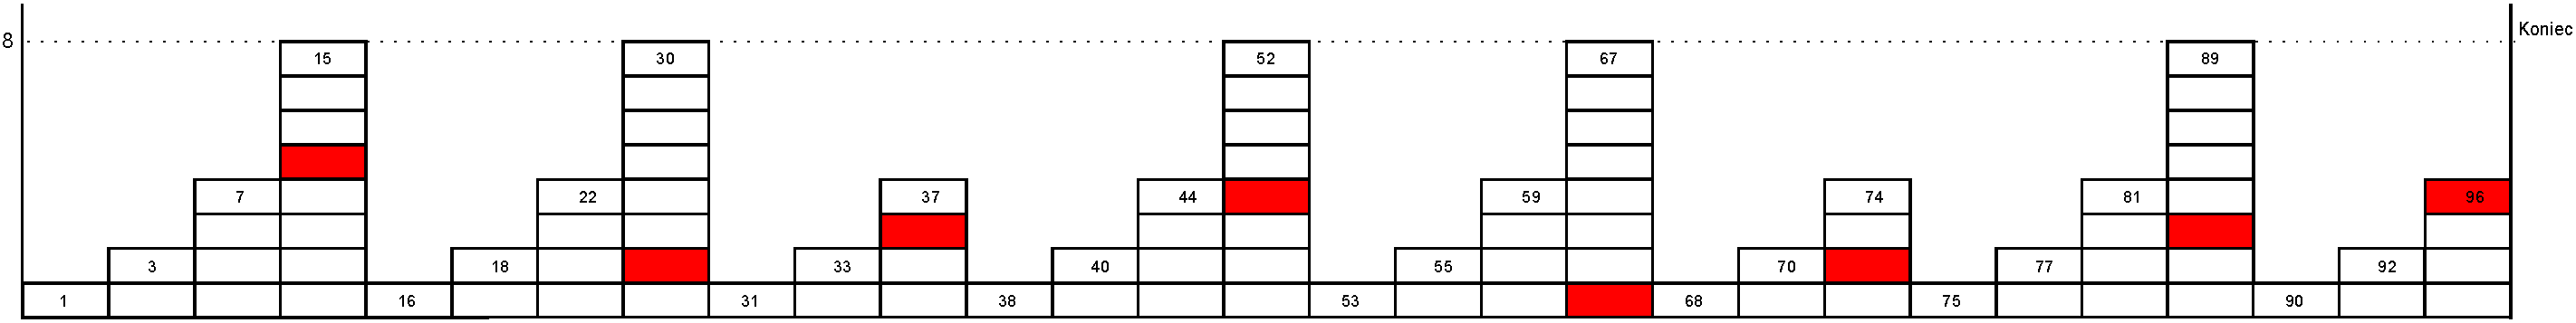
\includegraphics[width=16.0cm]{./images/zadanie08.pdf}\\\\
			Na 96 pakietów 8 zostaje przekłamanych.\\
			Możemy wyróżnić dwa parametry spełniające zadanie:
			\begin{enumerate}
				\item Szybkość efektywna: $ SRET=\frac{(96-8)\cdot 768\;[B]}{29\cdot 45\;[ms]}=\frac{88\cdot 768\;[B]}{29\cdot 45\;[ms]} $
				\item $ GND=\frac{(96-36)\cdot 768\;[B]}{29\cdot 45\;[ms]}=\frac{60\cdot 768\;[B]}{29\cdot 45\;[ms]} $
			\end{enumerate}
			\small{ \emph{Forczu: w tego typu zadaniach przepustowość chyba zawsze jest maksymalna, a protokoół standardowy, co ma upraszczać całość.
			Ktoś tam napisał, że wielkość ramki we wzorach jest obojętna, ale należy zaznaczyć, czy bierzemy dane czy dane + narzut.}}.
	% ================= ZADANIE 3 ==================
	\subsection{Zadanie}
		\subsubsection{Treść}
			Stacja robocza podłączona jest z serwerem łączem o przepustowości $ 55\;Mbit/s $, z bitową stopą błędów $ BER=4.9\cdot 10^{-6} $. określ, ile czasu zajmie przesłanie tym łączem pliku 100 kB danych, od nawiązania do zakończenia połączenia protokołem TCP w wersji standardowej, jeśli uzgodniona maksymalna wielkość segmentu wynosi 1024 B (ramki o łączu 1082 B), wielkość okna odbiorcy wynosi 17 kB, a czas RTT wynosi 25 ms.
		\subsubsection{Odpowiedź}
			$ BER=4.9\cdot 10^{-6} $
			\begin{itemize}
				\item Oznacza to, że 4.9 bitu zostaje przekłamanych na 1 milion bitów.
				\item Czyli 4.9 bajtów zostaje przekłamanych na 125000 bajtów.
				\item $ \cfrac{\frac{125\;000}{4.9}}{1082}\approx 23.58 $ - co 24 ramka jest przekłamana.
			\end{itemize}
			TODO: uzupełnić tej szajs analogicznie.
	% ================= ZADANIE 4 ==================
	\subsection{Zadanie}
		\subsubsection{Treść}
			W systemie transmisji posługującym się protokołem SDLC (tryb NRM, w=3, retransmisja grupowa) w łączu ze stopą błędów $ p=10^{-4} $ przesyłane są dane ramkami z polem danych 256 B, ze stacji nadrzędnej do stacji podrzędnej. Przedstaw przebieg transmisji w przesyle \textbf{4.5 kB} danych, pomiń nawiązanie / zrywanie połączenia. Ile kosztuje (narzut protokołu) obsługa błędów w transmisji?
		\subsubsection{Odpowiedź}
			Najpierw liczymy ilość potrzebnych ramek
			$$ \cfrac{4.5\;kB}{256\;B}=18\;[ramek] $$
			Następnie należy wyliczyć, co którą ramkę pojawi się przekłamanie. Stopa błędu wynosi 1/10000, czyli to oznacza, że co 10000 bit następuje przekłamanie, co równa się 1250 B. Teraz należy oblicz, co którą ramkę następuje błąd (i teraz nie jestem pewien ale chyba do tych 256 B danych należy dodać 6B nagłówka).
			$$ \cfrac{1250}{262}={4.77}\approx5 $$
			Co piąta ramka zawiera przekłamanie. Teraz można zacząć przedstawiać przebieg transmisji. "w" oznacza ile ramek możemy przesłać w takiej jednej sekwencji.\\
			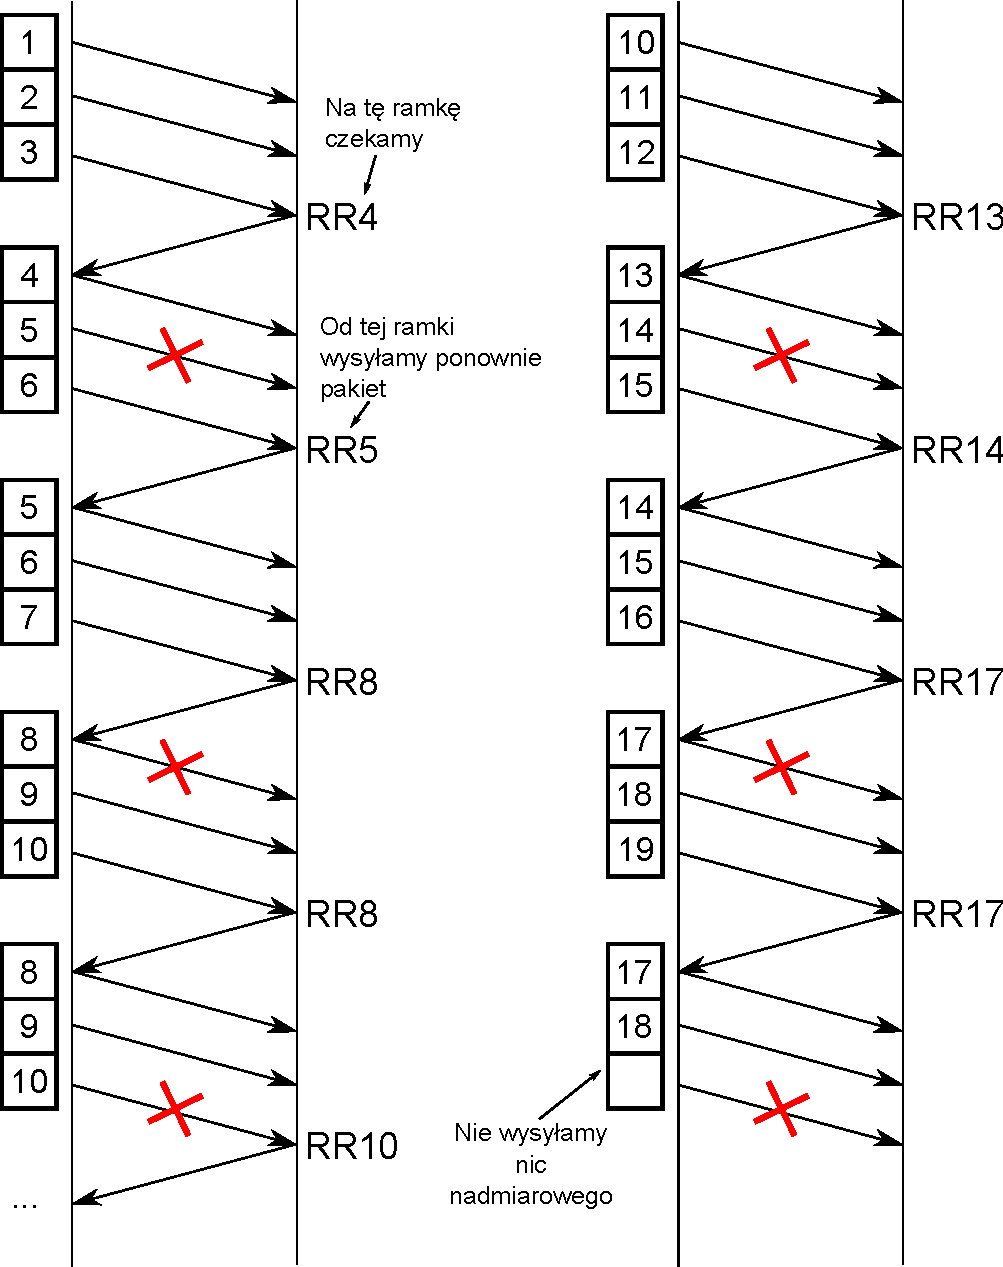
\includegraphics[width=9.0cm]{./images/zadanie09.pdf}\\\\
			Następnie należy policzyć narzut (ilość wszystkich ramek - ilość wymaganych ramek)\\
			$$ Narzut = 28 - 18  = 10\;ramek = 10 * 256\;B = 2560\;B $$
			\small{ \emph{Forczu: ocenione na 1.0 / 1.0}}.
	% ================= ZADANIE 5 ==================
	\subsection{Zadanie}
		\subsubsection{Treść}
			W systemie z protokołem SDLC (tryb NRM, w=3, retransmisja grupowa), ze stopą błędów $ p=10^{-4} $, ramki są wysyłane z polem danych 256 B ze stacji nadrzędnej do podrzędnej. Przedstaw przebieg transmisji przy przesyle \textbf{4 kB} danych. Pomiń nawiązanie i zerwanie połączenia. Ile kosztuje (narzut protokołu) obsługa błędów w transmisji?
		\subsubsection{Odpowiedź}
			1 błąd co 10 000 bitów $ \rightarrow $ 1 błąd do 1250 bajów $ \rightarrow $ 1 błąd w przybliżeniu co 5 ramek.\\
			$$ \cfrac{4\;[kB]}{256\;[B]}=16\;[ramek] $$
			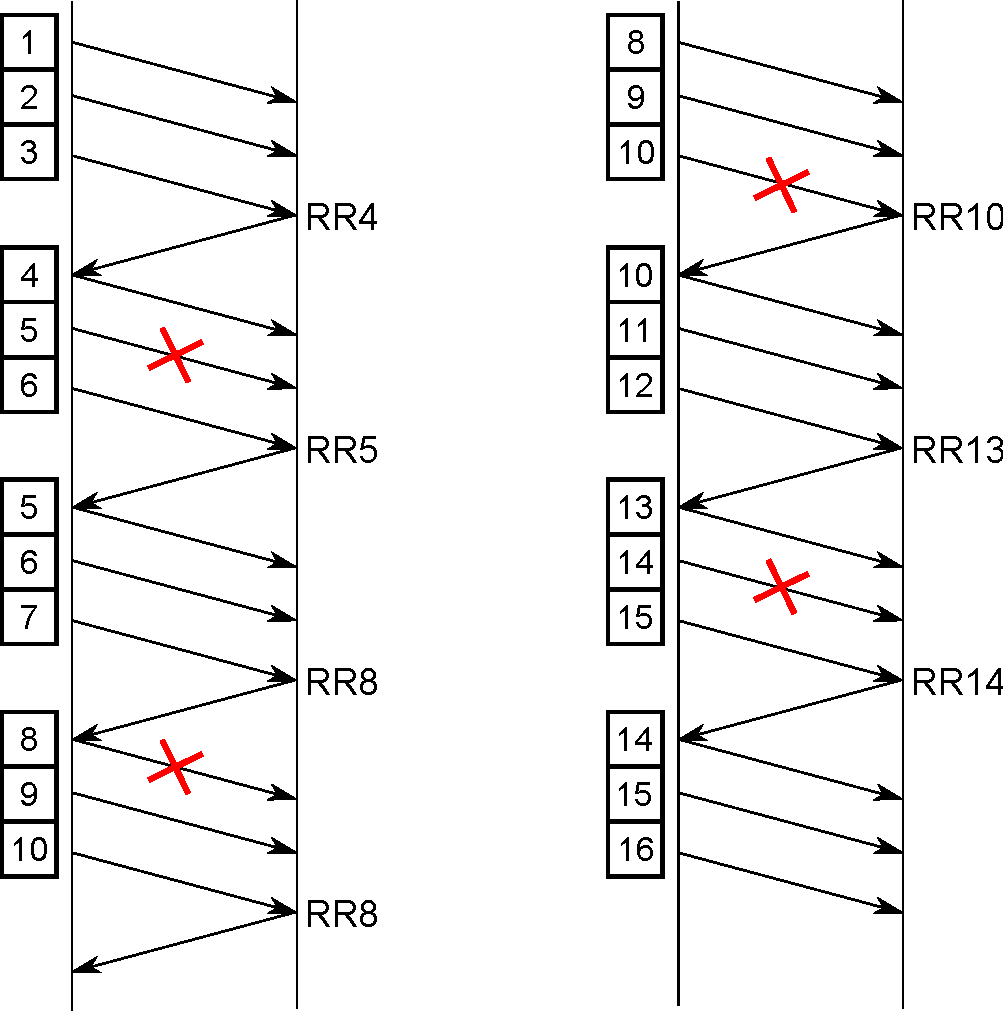
\includegraphics[width=8.0cm]{./images/zadanie10.pdf}\\\\
			Wysłaliśmy łącznie 24 ramki. Narzut: 24 - 16 = 8 ramek = 2048 B
	% ================= ZADANIE 6 ==================
	\subsection{Zadanie}
		\subsubsection{Treść}
			W systemie transmisji z protokołem HDLC średnio jeden na 9000 bitów jest przekłamany. Jaki będzie koszt obsługi błędów transmisji przy przesyle bloku 4 kB danych ze stacji B do stacji A w tym systemie, jeśli wielkość pola danych to 256 B, okno w=4, tryb NRM z retransmisją grupową.
		\subsubsection{Odpowiedź}
			$$ \cfrac{4\;[kB]}{256\;[B]}=16\;[ramek] $$
			$ \cfrac{1}{9000} $ bitów przekłamanych $ \rightarrow \cfrac{1}{1125}\;[B] \rightarrow $ co 5 ramka przekłamana.\\\\
			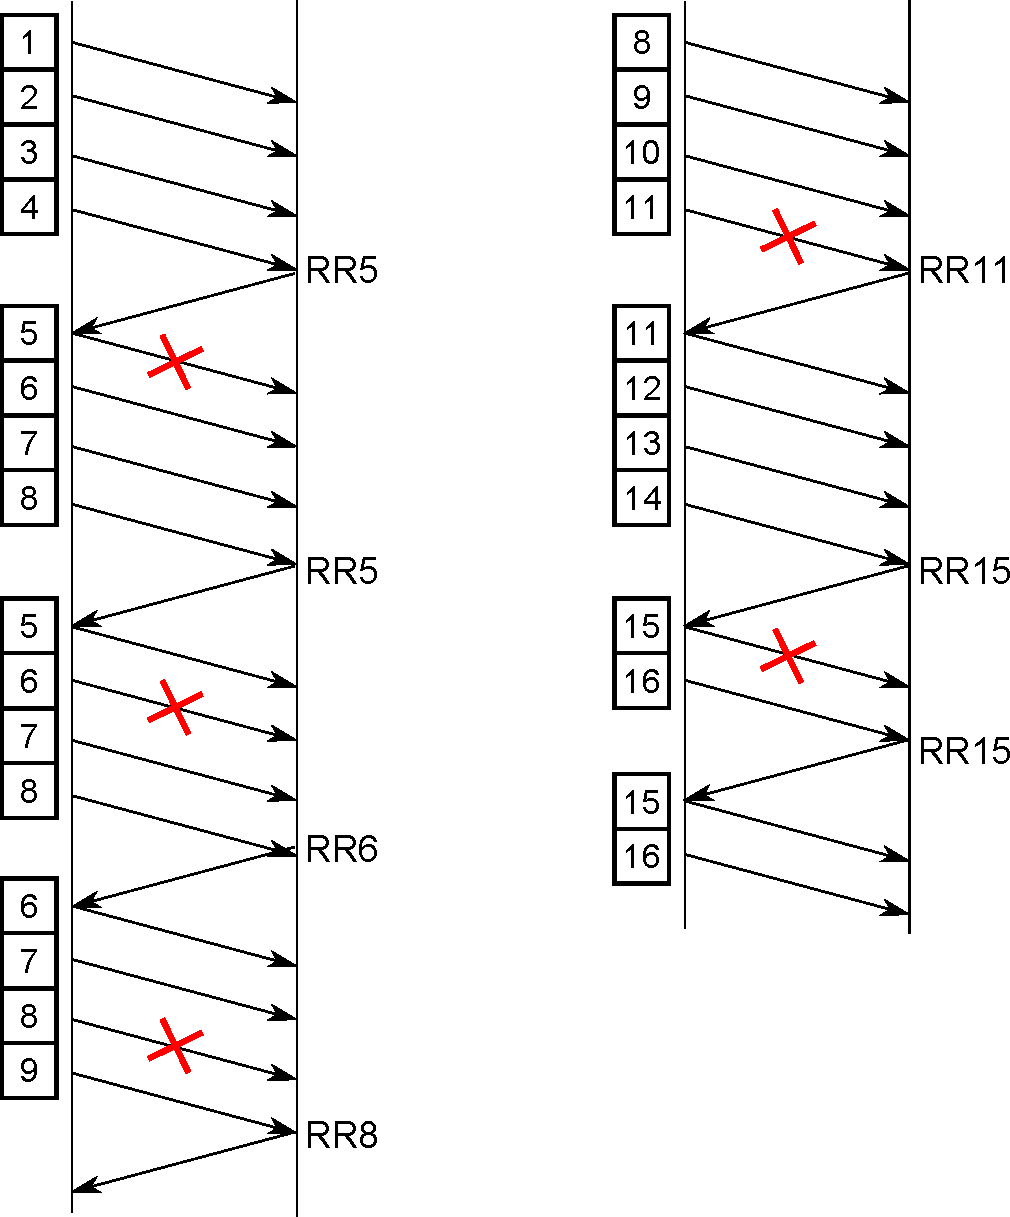
\includegraphics[width=8.0cm]{./images/zadanie12.pdf}\\\\
			Wysłano 28 ramek. Narzut: 28 - 16 = 12 ramek = 3 kB = 3072 B.
	% ================= ZADANIE 7 ==================
	\subsection{Zadanie}
		\subsubsection{Treść}
			Chcemy zastosować protokół CSMA / CD przy budowie sieci o długości łącza 500 m przy szybkości transmisji 200 MBit/s. Jaka powinna być w tym przypadku minimalna długość ramki?
		\subsubsection{Odpowiedź}
			Najpierw liczymy czas propagacji $$ t_p = \cfrac{dystans}{predkosc\_lacza} $$
			Prędkości łącza nie mylić z szybkością transmisji. W przypadku światłowodu wynosi ono 2/3 prędkości światła czyli 200 000 000 m/s, tu takie założenie można dać.
			$$ t_p=\frac{500\;[m]}{200\:000\:000\:[m/s]}=2.5\:\mu s $$
			Następnie wyliczamy długość ramki
			$$ N=szybkosc\_transmisji\cdot t_p $$
			Razy dwa ponieważ "Istnieje możliwość, że dwa lub więcej urządzeń przystąpi do wysyłania danych w tej samej chwili lub zanim sygnał z pierwszego węzła dotrze do drugiego. W takiej sytuacji żadne z nich nie wykryje sygnału nośnego drugiego. W efekcie obydwa urządzenia wysyłając dane w (prawie) tym samym czasie spowodują kolizję w sieci Ethernet."
			$$ N=200\:000\:000\:[bit]\cdot \frac{5}{10^6} =200\cdot5=1000\:bit=125\:B $$
						
	% ================= ZADANIE 6 ==================
	\subsection{Zadanie}
		\subsubsection{Treść}
			Węzeł W ma za sąsiadów węzły A, B, C, D i E. Po otrzymaniu pakietu Link State węzeł oczekuje 35 ms, następnie przystępuje do dystrybucji pakietu. W chwili $ t_0 $ węzeł odebrał pakiet z węzła B, $ 5\;ms $ później z węzła D, a po 13 $ ms $ pakiet z węzła E. Przedstaw przebieg dystrybucji pakietów\\.
			\begin{tabular}{|c|c|c|c|c|c|c|c|}
				\hline \multicolumn{2}{|c|}{\textbf{E}}  & & \multicolumn{2}{|c|}{\textbf{B}} & & \multicolumn{2}{|c|}{\textbf{D}}\\ 
				\hline \multicolumn{2}{|c|}{55} & &\multicolumn{2}{|c|}{55} & &\multicolumn{2}{|c|}{55} \\ 
				\hline \multicolumn{2}{|c|}{240} & &\multicolumn{2}{|c|}{238} & &\multicolumn{2}{|c|}{239}   \\ 
				\hline U & 2 & & U & 1 & & U & 2\\ 
				\hline V & 3 & & V & 2 & & V & 3\\
				\hline Z & 6 & & Z & 5 & & Z & 6\\
				\hline 
			\end{tabular}
		\subsubsection{Odpowiedź}
			Do węzłów, których pakiety miały największy nr sekwencyjny (2gi wiersz) wysyła potwierdzenie
			Do pozostałych wysyła pakiet tego węzła, który miał największy nr sekwencyjny i age (3ci wiersz).
			\begin{itemize}
				\item Do węzła D wyśle: potwierdzenie.
				\item Do węzła C wyśle: E.
				\item Do węzła B wyśle: potwierdzenie.
				\item Do węzła E wyśle: potwierdzenie.
				\item Do węzła A wyśle: E.
			\end{itemize}
	% ================= ZADANIE 7 ==================
	
			

\section{Adresacja}
	% ================= ZADANIE 1 ==================
	\subsection{Zadanie}
		\subsubsection{Treść}
			Jak przebiega (po raz pierwszy w danych środowisku) proces tłumaczenia nazwy na adres IP dla nazwy daisy.sales.euro.hp.com? Czy zwracany wynik i proces tłumaczenia różni się czymś przy drugiej próbie w stosunku do pierwszej (odstęp między żądaniami kilka minut, pierwsza zakończona pomyślnie)? Jak będzie przebiegał późniejszy o kilka minut proces tłumaczenia nazwy dino.support.americas.hp.com?
		\subsubsection{Odpowiedź}
			\begin{enumerate}[A]
				\item 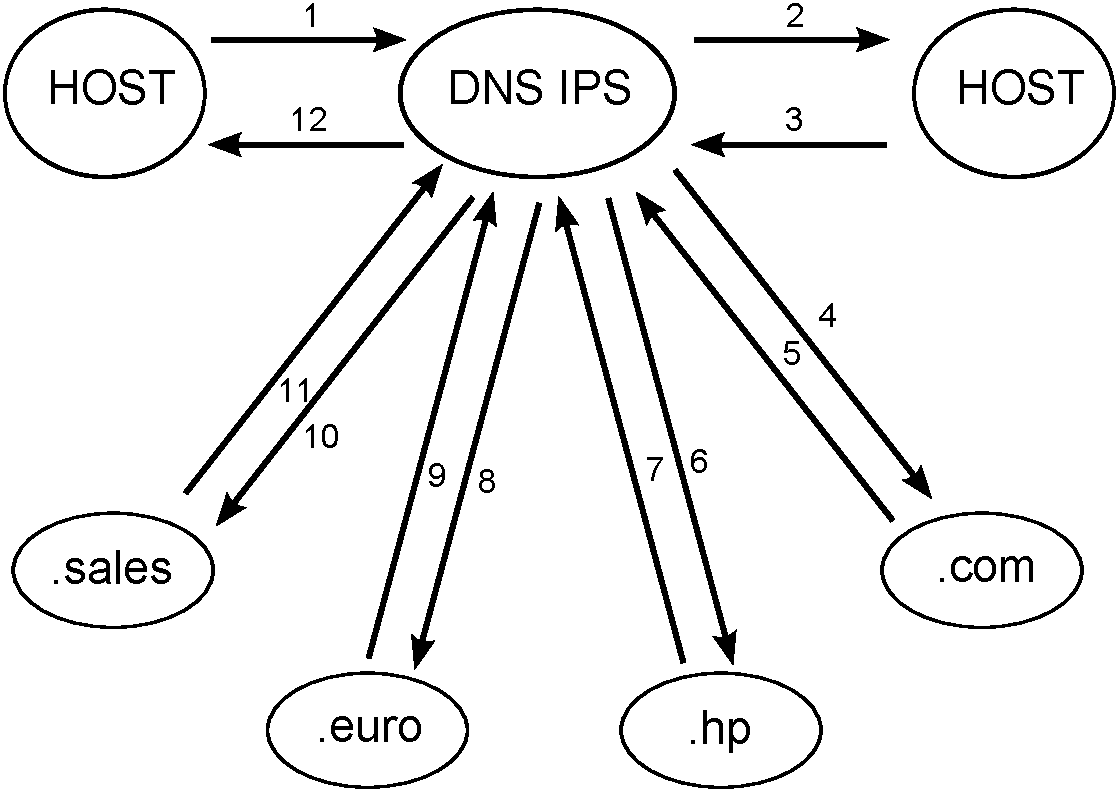
\includegraphics[width=6cm]{./images/zadanie01.pdf}\\
				\begin{enumerate}[1]
					\item Zapytanie DNS o adres IP dla daisy.sales...
					\item Jeśli DNS nie posiada tego adresu to pyta root server
					\item Ten odpowiada, że nie zna adresu IP dla daisy.sales.euro.hp.com , ale zna adres dla com i ... (przekierowuje)
					\item DNS ISP pyta dns com o daisy.sales.euro.hp.com
					\item Ten odpowiada, że go nie zna, ale zna adres dla hp
					\item DNS ISP pyta dns hp o daisy.sales.euro.hp.com
					\item Ten odpowiada, że go nie zna, ale zna adres dla euro
					\item DNS ISP pyta dns euro o daisy.sales.euro.hp.com
					\item Ten odpowiada, że go nie zna, ale zna adres dla sales
					\item DNS ISP pyta dns sales o daisy.sales.euro.hp.com
					\item Serwer sales zwraca adres IP domeny daisy.sales.euro.hp.com. Następnie DNS ISP p(...) go do hosta.
					\item ...
				\end{enumerate}
				\small{ \emph{Brak pełnej treści, ale ocenione na 1.0 / 1.0}}
				\item
					\begin{enumerate}
						\item daisy.sales.euro.hp.com.root
						\begin{enumerate}[1]
							\item Zapytanie do NS .com czy "zna" .hp
							\item Zapytanie do NS .hp czy zna .euro
							\item Zapytanie do NS .euro czy zna .sales
							\item Zapytanie do NS .sales czy zna .daisy
							\item Otrzymanie adresu IP
						\end{enumerate}
						W drugim przypadku adres hp.com może nie być tłumaczony.
						\item dino.support.americas.hp.com
						\begin{enumerate}[1]
							\item Znamy IP (hp.com), pytamy czy zna .americas
							\item Zapytanie do NS czy zna .support
							\item Zapytanie do NS czy zna .dino
							\item Otrzymanie adresu IP
						\end{enumerate}
					\end{enumerate}
					\small{ \emph{Ocenione na 1.0 / 1.0}}
			\end{enumerate}
	% ================= ZADANIE 2 ==================
	\subsection{Zadanie}
		\subsubsection{Treść}
			Dostępna jest pewna ilość kolejnych adresów internetowych, zaczynając od 192.170.0.0. Cztery organizacje A, B, C i D występowały kolejno o przydział puli 1000, 2000, 4000 i 1000 adresów IP. Podaj dla każdej z nich pierwszy i ostatni przyznany adres oraz maskę sieci w notacji w.x.y.z i /m.
		\subsubsection{Odpowiedź}
			W treści zadania jest podane, że te firmy przychodziły \textit{kolejno}, więc po prostu w tej kolejności przyznajemy im adresy.
			\begin{enumerate}
				\item Firma A, 1000 adresów - maska na 1024 adresy
				\begin{itemize}
					\item Pierwszy adres: 192.170.0.0
					\item Ostatni adres: 192.170.3.255
					\item w.x.y.z: 255.255.252.0 (1.1.11111100.0)
					\item Maska: /22
				\end{itemize}
				\item Firma B, 2000 adresów - maska na 2048 adresy
				\begin{itemize}
					\item Nie możemy w połowie wstawić takiej maski, minimalny przydział takiej podsieci jest „co 2048”. Innymi słowy musimy zostawić przerwę po pierwszej podsieci o długości 1024 adresy, by wyrównać je do 2048.
					\item Pierwszy adres: 192.170.8.0
					\item Ostatni adres: 192.170.15.255
					\item w.x.y.z: 255.255.248.0 (1.1.11111000.0)
					\item Maska: /21
				\end{itemize}
				\item Firma C, 4000 adresów - maska na 4096 adresy
				\begin{itemize}
					\item Pierwszy adres: 192.170.16.0
					\item Ostatni adres: 192.170.31.255
					\item w.x.y.z: 255.255.240.0 (1.1.11110000.0)
					\item Maska: /20
				\end{itemize}
				\item Firma D, 1000 adresów - maska na 1024 adresy
				\begin{itemize}
					\item Mamy wolne miejsce między podsieciami dla firmy A i B, tam dajemy tę sieć.
					\item Pierwszy adres: 192.170.4.0
					\item Ostatni adres: 192.170.7.255
					\item w.x.y.z: 255.255.252.0 (1.1.11111100.0)
					\item Maska: /22
				\end{itemize}
			\end{enumerate}
	% ================= ZADANIE 3 ==================
	\subsection{Zadanie}
		\subsubsection{Treść}
			Firma dysponuje pulą 32 adresów IP. Przyjęto, że pierwszy i ostatni użyteczny adres zostaną przydzielone routerowi dostępowemu i serverowi DNS. Jeden z komputerów otrzymał adres 172.19.21.137. Podaj elementy konfiguracji IP tego komputera.
		\subsubsection{Odpowiedź}
			\begin{itemize}
				\item \textbf{Maska podsieci}: 255.255.255.224 (albo /27)\\
				Firma posiada 32 adresy, które różnią się 5 najmłodszymi bitami. 32 - 5 = 27.
				\item \textbf{Adres IP}: 172.19.21.137
				\item \textbf{Host}: 172.19.21.128 /27 (adres sieci)\\
				Adresem sieci wyliczamy zerując 5 ostatnich bitów. (albo ANDując adres z 1.1.1.11100000)
				\item \textbf{Brama / Router}: 172.19.21.129\\
				Adres routera dostępowego, pierwszy użyteczny adres (00001).
				\item \textbf{Serwer DNS}: 172.19.21.158\\
				Ostatni użyteczny adres (11110). (Broadcast - 1)
				\item \textbf{Broadcast}: 172.19.21.159\\
				Adres rozgłoszeniowy, uzyskany przez "zajedynkowanie" 5 ostatnich bitów. Największy adres w sieci.
				\item Adresy przydzielamy wg kolejnych potęg dwójki $ 2^n $. Gdyby w treści były 33 adresy, to przydzielalibyśmy 64.
				\item Gdyby w treści należałoby podpiąć 32 klientów, to musielibyśmy mieć 34 adresy i znów przydzielać 64.
			\end{itemize}
	% ================= ZADANIE 4 ==================
	\subsection{Zadanie}
		\subsubsection{Treść}
			
		\subsubsection{Odpowiedź}	
			
	
\section{Poczta e-mail}
	% ================= ZADANIE 1 ==================
	\subsection{Zadanie}
		\subsubsection{Treść}
			Przedstawić z jakich elementów składa się koperta przesyłki poczty elektronicznej.
			\begin{enumerate}[a)]
				\item Jak przebiega i który z protokołów poczty elektronicznej odpowiada za jej przekazanie?
				\item Jak przebiega odbiór przesyłki przez adresata, który z protokołów obsługuje tę operację?
			\end{enumerate}
		\subsubsection{Odpowiedź}
			\begin{enumerate}[a)]
				\item List elektroniczny wysyłany jest za pomocą protokołu SMTP. Klient inicjuje połączenie poleceniem "helo". Następnie podaje adres nadawcy "mail from", adres odbiorcy "rcpt to", treść listu "data". 
				\\(Koniec części z danymi oznacza pusta linia z '.'. - \textit{doxus}) 
				\\Wiadomość kończy poleceniem "quit".
				\item Listy odbierane są za pomocą protokołów POP3. Klient żąda listy wiadomości poleceniem "list". Następnie pobiera cały żądany list i usuwa go z serwera : "Retr" i "Dele". Sesja kończy się poleceniem "quit". Oczywiście zanim to wszystko nastąpi musi zostać przeprowadzona autentyfikacja. Klient POP3 zaczyna sesję od podania nazwy użytkownika "user" i hasła "pass".
			\end{enumerate}
			\small{ \emph{Ocenione na 1.0 / 1.0}}
